\documentclass [12pt,a4paper] {article}
\usepackage[usenames]{color}
\usepackage{graphicx}
\usepackage{amssymb, amsmath, amsbsy}
\usepackage[utf8]{inputenc}
\usepackage[breaklinks=true]{hyperref}
\hypersetup{
    colorlinks=true,
    linkcolor=blue,
    filecolor=magenta,      
    urlcolor=cyan,
    final=true,
}
\urlstyle{same}

% Inicio de documento
\title{ Ejemplo de texto en LaTeX}
\author{ Juan Manuel Mena }
\begin{document}
\maketitle 
\LaTeX{} es muy potente, puedes escribir formulas matematicas muy facilmetente.
\textbf{Ejemplos: }

\begin{displaymath}
  E= m c^2 
\end{displaymath}

Podemos usar color en este tipo de documentos:

\textcolor{cyan}{texto}

\textcolor{magenta}{texto}

Otra opcion es usar listas:

\begin{itemize}
    \item Madrid.
    \item Castilla la Mancha.
    \item Castilla y León.
    \begin{itemize}
         \item Segovia.
         \item Ávila.
    \end{itemize}
\end{itemize}

Una funcion interesante es su uso para escribir reacciones quimicas:

\begin{equation}
D \rightarrow E\uparrow + F\downarrow
\end{equation}

Podemos instertar tablas:

\vspace{5mm}
\begin{tabular}{llcr}
\hline
pepino & tomate & berenjena & rábano  \\
\hline
manzana & naranja & fresa & pera \\
\hline
\end{tabular}

\vspace{5mm}

Nos permite dirigir a enlaces:

\vspace{5mm}
\href{ https://www.google.com }{Esto es un enlace a google} 
\vspace{5mm}

Tambien podemos añadir imagenes dentro de este tipo de archivo:

\begin{figure}
\centering
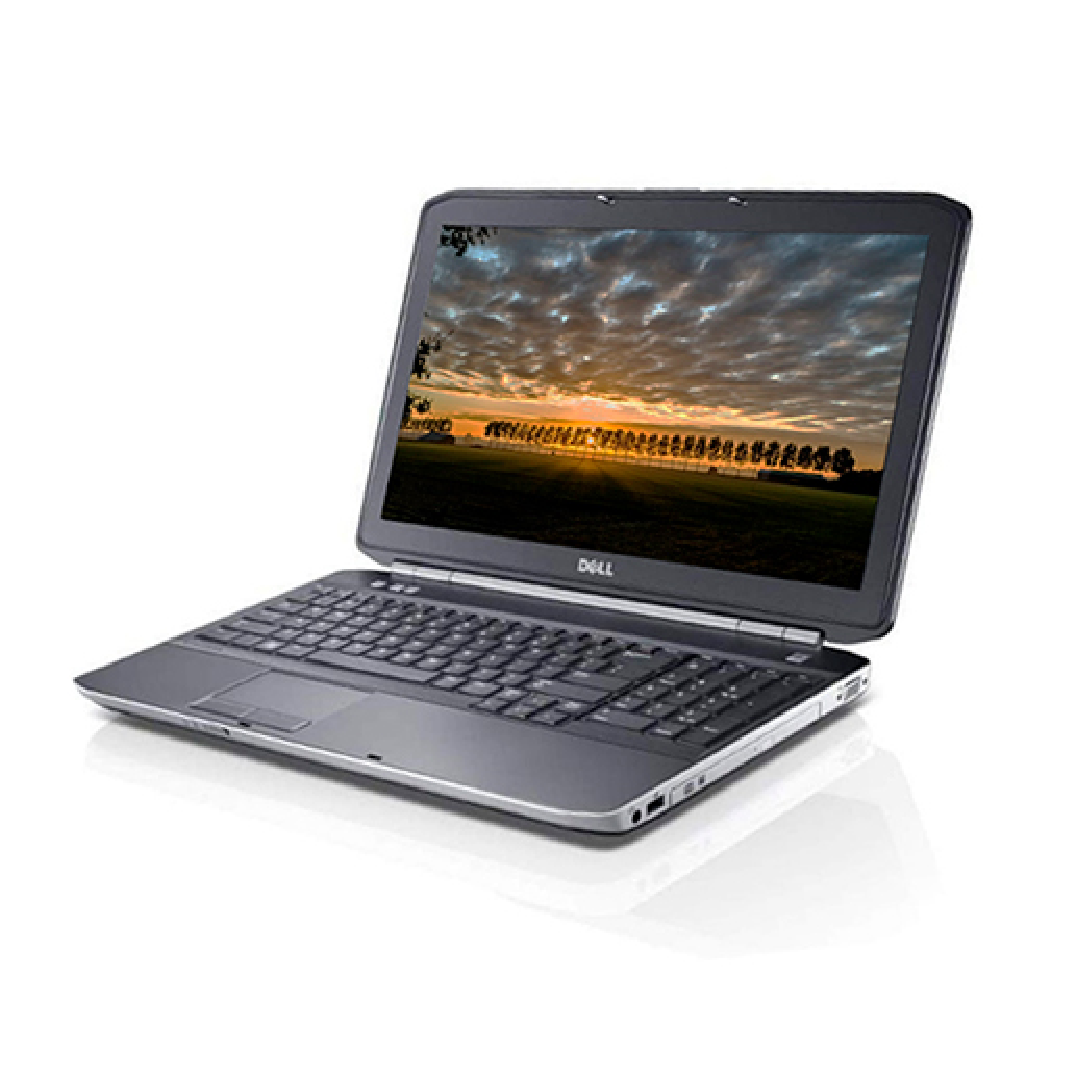
\includegraphics[width=0.8\textwidth]{./dell}
\caption{Portatil.} \label{fig:Dell}
\end{figure}


\end{document}

